% Author: Damanic Luck
% Email: damanicluck@berkeley.edu
% CSM16A Spring 2023

\qns{2D Resistive Touchscreen}

\textbf{Learning Goal: } Understand how a 2D resistive touchscreen works and how to translate the touchpoint to a real coordinate position

Since the last week with your 1D resistance touchscreen, you decided that you want to make yourself something even cooler: a drinks dispenser controller. In this worksheet, you'll be making yourself a 2D resistive touchscreen that will dispense you a specific drink depending based on where you touch the 2D resistive touchscreen. This picture below will model the 3 by 3 square touchscreen you will be creating in this problem!
    \begin{center}
        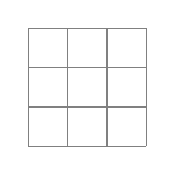
\begin{tikzpicture}
            \draw[step=0.5 cm,color=gray] (0,0) grid (1.5,1.5);
        \end{tikzpicture}
    \end{center} 
Please review \href{https://eecs16a.org/lecture/Note14.pdf}{Note 14} for a physical model of the 2D resistive touchscreen. You want to build a square resistive touchscreen with the options to select 9 drinks. Therefore, you'll be needing 6 resistor strips to form a grid structure like the one below. Assume that your resistor strips are of uniform width, length, and spacing between the them. Concepts from the 1D resistive touchscreen still apply! 
    \begin{center}
        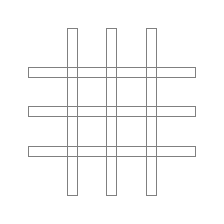
\begin{tikzpicture}
            \draw [draw=gray, very thin] (0,0)   rectangle ++(0.125,2.125);
            \draw [draw=gray, very thin] (0.5,0) rectangle ++(0.125,2.125);
            \draw [draw=gray, very thin] (1,0)   rectangle ++(0.125,2.125);
            \draw [draw=gray, very thin] (-0.5, 0.5) rectangle ++(2.125, 0.125);
            \draw [draw=gray, very thin] (-0.5, 1) rectangle ++(2.125, 0.125);
            \draw [draw=gray, very thin] (-0.5, 1.5) rectangle ++(2.125, 0.125);
        \end{tikzpicture}
    \end{center}

Notice how the overlapping areas of the 6 strips correspond to the 3 by 3 grid above!

\meta {
    Make sure to clarify that they can measure touch because of the resulting voltage that occurs at a particular node
    \begin{itemize}
        \item Voltage dividers are extremely important to circuit analysis
        \item \textbf{Use voltage dividers to get voltages in the x and y direction to get voltages that correspond to locations}
    \end{itemize}
}

\begin{enumerate}
    % part (a)
    \item Find the voltage for the $V_{out}$ as a function of $R_{touch}$, $R_{rest}$, and $V_s$.
        \begin{center}
            \begin{circuitikz}[american]
                \draw
                    (0,0) to [vsource, l=$V_s$, invert] ++(0,4)
                    to [short] ++(2, 0)
                    to [R, l_=$R_{rest}$] ++(0,-2)
                    to [R, l_=$R_{touch}$] ++(0, -2)
                    to ++(-2,0) node[ground]{};
                \draw 
                    (2, 2) to [short, -*] ++ (1, 0)
                    to [open, l=$V_{out}$] ++(0,-2)
                    to [short, *-] ++(-1,0);
            \end{circuitikz}
        \end{center}
    \meta {Emphasize voltage dividers since this will come in use later when they are analyzing part(d). This should not actually take that long for them to do.}

        \ans {
            Notice how this is simply a voltage divider! So,
                \begin{align*}
                    V_{out} = V_s \bigg( \frac{R_{touch}}{R_{touch}+R_{rest}}\bigg)
                \end{align*}
            }
    
    % part (b)
    
    \item Moving on! How do voltage dividers even relate to how we are building this circuit anyways? (That's a rhetorical question.) \\
    
    Given the circuit below that models finding the \textbf{y} direction, does it actually matter whether we replace $R_1$ and $R_1$ with open circuits? Find the equation for the voltages at each node, $u_{iy}$, as a function of $V_s, R_{touch}$, and $R_{rest}$. \emph{Hint: How can you utilize part(a) here?}\\
    \meta{They will be finding voltage in the y direction first because its easier to visualize since that looks like the voltage divider the most. \textbf{Emphasize that it looks like a voltage divider.}}
        \begin{center}
            \begin{circuitikz}[american, scale=0.8]
                \draw
                    node[ground]{} (0,0) to [vsource,l=$V_s$,invert] ++(0,8)
                    to [short] ++(6,0)
                    to [short, -*] ++(0,-1) 
                        node[label={[font=\footnotesize] 45:$u_{2y}$}]{}
                    to [R, l=$R_{rest}$, -*] ++(0,-3) 
                        node[label={[font=\footnotesize] 45:$u_{5y}$}]{}
                    to [R, l=$R_{touch}$, -*] ++(0,-3)
                        node[label={[font=\footnotesize] 45:$u_{8y}$}]{}
                    to [short] ++(0,-1)
                    to [short] ++(-6,0);
                    \draw
                    (3,7) to [short, -*] ++(6,0)
                        node[label={[font=\footnotesize] 45:$u_{3y}$}]{}
                    to [R, l=$R_{rest}$, -*] ++(0,-3) 
                        node[label={[font=\footnotesize] 45:$u_{6y}$}]{}
                    to [R, l=$R_{touch}$, -*] ++(0,-3)
                        node[label={[font=\footnotesize] 45:$u_{9y}$}]{}
                        to [short, -*] ++(-6,0)
                        node[label={[font=\footnotesize] 45:$u_{7y}$}]{}
                    to [R, l=$R_{touch}$, -*] ++(0,3)
                        node[label={[font=\footnotesize] 45:$u_{4y}$}]{}
                    to [R, l=$R_{rest}$, -*] ++(0,3)
                        node[label={[font=\footnotesize] 45:$u_{1y}$}]{};
                \draw
                    (3,4) to [R=$R_1$] ++(3,0)
                    to [R=$R_2$] ++(3,0);
                \end{circuitikz}
            \end{center}
        \ans {
            No, it doesn't matter whether $R_1$ and $R_2$ are replaced with open circuits because the voltage at $u_4, u_5,$ and $u_6$ are the \textbf{same}, as long as $R_{rest}$ is still the same. Because of this, there is no current flow between these nodes so it can be equivalently represented as an open circuit. The circuit diagram below demonstrates this. Notice how it resembles three separate voltage dividers! You can solve for the voltages at $u_4, u_5$, and $u_6$. \\
            \begin{center}
                \begin{circuitikz}[american, scale=0.8]
                    \draw
                        node[ground]{} (0,0) to [vsource,l=$V_s$,invert] ++(0,8)
                        to [short] ++(6,0)                            to [short, -*] ++(0,-1) 
                            node[label={[font=\footnotesize] 45:$u_{2y}$}]{}
                        to [R, l=$R_{rest}$, -*] ++(0,-3) 
                            node[label={[font=\footnotesize] 45:$u_{5y}$}]{}
                        to [R, l=$R_{touch}$, -*] ++(0,-3)
                            node[label={[font=\footnotesize] 45:$u_{8y}$}]{}
                        to [short] ++(0,-1)
                        to [short] ++(-6,0);
                    \draw
                        (3,7) to [short, -*] ++(6,0)
                            node[label={[font=\footnotesize] 45:$u_{3y}$}]{}
                        to [R, l=$R_{rest}$, -*] ++(0,-3) 
                            node[label={[font=\footnotesize] 45:$u_{6y}$}]{}
                        to [R, l=$R_{touch}$, -*] ++(0,-3)
                            node[label={[font=\footnotesize] 45:$u_{9y}$}]{}
                        to [short, -*] ++(-6,0)
                            node[label={[font=\footnotesize] 45:$u_{7y}$}]{}
                        to [R, l=$R_{touch}$, -*] ++(0,3)
                            node[label={[font=\footnotesize] 45:$u_{4y}$}]{}
                        to [R, l=$R_{rest}$, -*] ++(0,3)
                            node[label={[font=\footnotesize] 45:$u_{1y}$}]{};
                \end{circuitikz}
            \end{center}
             Intuitively, you know that since $u_1, u_2$, and $u_3$ are connected on the same node, they are equal to $V_s$ and the same logic applies for $u_7, u_8$, and $u_9$.\\
            \begin{align*}
                 u_{1y} &= u_{2y} = u_{3y} = V_s \\
                 u_{4y} &= u_{5y} = u_{6y} = V_s\bigg( \frac{R_{touch}}{R_{touch}+R_{rest}}\bigg) \\
                 u_{7y} &= u_{8y} = u_{9y} = 0
            \end{align*}
            }   
    % part (c)
    \item Given the circuit that models the \textbf{x} direction. Similarly, does it matter if whether $R_3$ and $R_4$ are there? Find the equation for the voltages at each node, $u_{ix}$, as a function of $V_s, R_{touch}$, and $R_{rest}$.
            \begin{center}
                \begin{circuitikz}[american, scale=0.9]
                    \draw
                        node[ground]{} (0,0) to [vsource, l_=$V_s$,invert] ++(12,0)
                        to [short] ++(0,4)
                        to [short, -*] ++(-3, 0) 
                            node[label={[font=\footnotesize] 45:$u_{6x}$}]{}
                        to [R, l=$R_{rest}$, -*] ++(-3,0) 
                            node[label={[font=\footnotesize] 45:$u_{5x}$}]{}
                        to [R, l=$R_{touch}$, -*] ++(-3,0)
                            node[label={[font=\footnotesize] 45:$u_{4x}$}]{}
                        to [short] ++(-3,0)
                        to [short] ++(0,-4);
                    \draw 
                        (9, 4) [short, -*] to ++(0,2)
                            node[label={[font=\footnotesize] 45:$u_{3x}$}]{}
                        to [R, l=$R_{rest}$, *-*] ++(-3,0)
                            node[label={[font=\footnotesize] 45:$u_{2x}$}]{}
                        to [R, l=$R_{touch}$, -*] ++(-3,0)
                            node[label={[font=\footnotesize] 45:$u_{1x}$}]{}
                        to [short] ++(0,-4)
                            node[label={[font=\footnotesize] 45:$u_{7x}$}]{}
                        to [R, l_=$R_{rest}$, *-] ++(3,0)
                            node[label={[font=\footnotesize] 45:$u_{8x}$}]{}
                        to [R, l_=$R_{touch}$, *-] ++(3,0)
                            node[label={[font=\footnotesize] 45:$u_{9x}$}]{}
                        to [short, *-] ++(0,2);
                    \draw 
                        (6, 2) to [R, l=$R_3$] ++(0,2)
                        to [R, l=$R_4$] ++(0,2);
                \end{circuitikz}
            \end{center}
        
        \ans {Similarly, it also doesn't matter whether the resistors $R_3$ and $R_4$ are there either, by the same reasoning as in the previous part! There is no voltage drop across those resistors, so therefore there is also no current flow through these resistors. An equivalent circuit diagram is redrawn below. 
            \begin{center}
                \begin{circuitikz}[american, scale=0.7]
                    \draw
                        node[ground]{} (0,0) to [vsource, l_=$V_s$,invert] ++(12,0)
                        to [short] ++(0,4)
                        to [short, -*] ++(-3, 0) 
                            node[label={[font=\footnotesize] 45:$u_{6x}$}]{}
                        to [R, l=$R_{rest}$, -*] ++(-3,0) 
                            node[label={[font=\footnotesize] 45:$u_{5x}$}]{}
                        to [R, l=$R_{touch}$, -*] ++(-3,0)
                            node[label={[font=\footnotesize] 45:$u_{4x}$}]{}
                        to [short] ++(-3,0)
                        to [short] ++(0,-4);
                    \draw 
                        (9, 4) [short, -*] to ++(0,2)
                            node[label={[font=\footnotesize] 45:$u_{3x}$}]{}
                        to [R, l=$R_{rest}$, *-*] ++(-3,0)
                            node[label={[font=\footnotesize] 45:$u_{2x}$}]{}
                        to [R, l=$R_{touch}$, -*] ++(-3,0)
                            node[label={[font=\footnotesize] 45:$u_{1x}$}]{}
                        to [short] ++(0,-4)
                            node[label={[font=\footnotesize] 45:$u_{7x}$}]{}
                        to [R, l_=$R_{rest}$, *-] ++(3,0)
                            node[label={[font=\footnotesize] 45:$u_{8x}$}]{}
                        to [R, l_=$R_{touch}$, *-] ++(3,0)
                            node[label={[font=\footnotesize] 45:$u_{9x}$}]{}
                        to [short, *-] ++(0,2);
                \end{circuitikz}
            \end{center}
        Notice how this simplified circuit also resembles voltage dividers, but sideways! Therefore, 
            \begin{align*}
                 u_{3x} &= u_{6x} = u_{9x} = V_s \\
                 u_{2x} &= u_{5x} = u_{8x} = V_s\bigg( \frac{R_{touch}}{R_{touch}+R_{rest}}\bigg) \\
                 u_{1x} &= u_{4x} = u_{7x} = 0
            \end{align*}
        }

    %part (d)
    \item Match the drinks and their voltages! Given that each resistor in the circuit diagram shown in part (b) and (c) is each 1k Ohms and that $V_s$ is 8V. Write your answer in the grid below, which corresponds to your 2D resistive touchscreen.\\

    Each drink will be given in coordinate form, $(x, y)$, with $x$ denoting the voltage in the $x$ direction and $y$ denoting the voltage in the $y$ direction. Let the variable $m$ represent the value of your middle nodes. \emph{Hint: First solve for each node voltage now that you are given real values.}

    Drinks:
    
    \begin{align*}
        \text{Orange Juice: } (0, V_s) \\
        \text{Red Bull: } (V_s, m) \\
        \text{Green Tea: } (V_s, 0) \\
        \text{Sprite: } (m, m) \\
        \text{Black tea: } (0, 0) \\
        \text{Apple juice: } (V_s, V_s) \\
        \text{Water: } (0, m) \\
        \text{Coffee: } (m, 0) \\
        \text{Milk tea: } (m, V_s) \\
    \end{align*}
    \begin{center}
        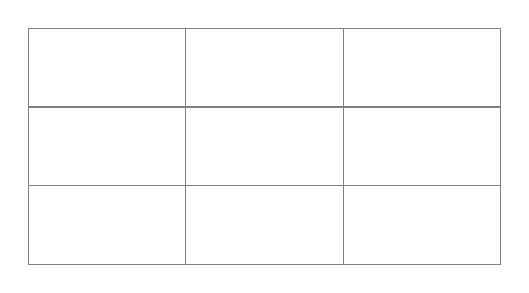
\begin{tikzpicture}
            \draw[xstep=2cm, ystep=1cm,color=gray] (0,0) grid (6,3);
        \end{tikzpicture}
    \end{center}
    
    \meta{ \textbf{Emphasize that the voltages they solve for can be used to directly determine location via a coordinate plane}}\\
    \ans{ First we should solve for each node voltage. Since we know that 2 sets of nodes will either be ground or equal to $V_s$, we only have to solve for the set of the middle nodes. Notice how the middle node values are equivalent to each other! Refer to the derived equations for the set of middle nodes in parts(b) and (c) for reference.
    \begin{align*}
        u_{4y} = u_{5y} = u_{6y} = u_{2x} = u_{5x} = u_{8x} &= V_s\bigg( \frac{R_{touch}}{R_{touch}+R_{rest}}\bigg) \\
        &= 8V \bigg( \frac{1k\si\Omega}{1k\si\Omega+1k\si\Omega} \bigg) \\
        &= 4V
    \end{align*}
    For easy reference, here are the values that correspond to each node:
    \begin{align*}
        u_{1y} &= u_{2y} = u_{3y} = u_{3x} = u_{6x} = u_{9x} = 8V \\
        u_{4y} &= u_{5y} = u_{6y} = u_{2x} = u_{5x} = u_{8x} = 4V \\
        u_{7y} &= u_{8y} = u_{9y} = u_{1x} = u_{4x} = u_{7x} = 0V
    \end{align*}
    
    The following matrix corresponds to the grid above.
    %i could not for the life of me understand how to put text in grids with an anuerysm
    \begin{center}
        \begin{bmatrix}
            \text{Orange juice} & \text{Milk tea} & \text{Apple juice} \\
            \text{Water} & \text{Sprite} & \text{Red Bull} \\
            \text{Black tea} & \text{Coffee} & \text{Green tea}
        \end{bmatrix}
    \end{center}
    }

    \item{Suppose your good friend Bob miraculuously messes up your new 2D resistive touchscreen. One of the resistor values has been swapped out for a value twice its original value! How will this impact your touchscreen? \\
    \meta{This question is here to show what happens if resistor values are not all the same.}\\
        \ans{
        Because of Bob's mistake, you no longer have no voltage drop across the the horizontal resistors in the middle between $u_{4y}$ and/or $u_{5y}$ and/or $u_{6y}$. This was a crucial design parameter for us to solve for the node voltages! Now your 2D resistive touchscreen can't be used as effectively as before. 
        }
    }
\end{enumerate}


\begin{comment}
This is the planning process for the worksheet.
PROPOSED STRUCTURE FOR THE QUESTIONS
1. intro about how youre making a drinks dispenser
(a) deriving equations for resistance
(b) deriving equation for the vertical position given the circuit representation
(c) horizontal
(d) matching the drinks to the position the resistive touchscreen
(e) bob comes to f up the day
\end{comment}